j\chapter{Apprentissage par le pratique}
\pagebreak

\section{Rappel}
\subsection{Matrices et calcules sur les Matrices}

\subsubsection{Addition}

$\left(\begin{array}{cc}
1 & 3 \\ 1 & 0 \\ 1 & 2 \end{array} \right)$
+
$\left(\begin{array}{cc}
0 & 0 \\ 7 & 5 \\ 2 & 1 \end{array} \right) $
=
$\left(\begin{array}{cc}
1+0 & 3+0 \\ 1+7 & 0+5 \\ 1+2 & 2+1 \end{array} \right) $
=
$\left(\begin{array}{cc}
1 & 3 \\ 8 & 5 \\ 3 & 3 \end{array} \right) $

\subsubsection{Multiplication}

$\begin{array}{c@{\ }c}
&
\left(\begin{array}{cc}
5 & 6 \\ 7 & 8 \end{array} \right) \\[0.5cm]
\left(\begin{array}{cc}
1 & 2 \\ 3 & 4 \end{array} \right)
&
\left(\begin{array}{cc}
19 & 22 \\ 43 & 50 \end{array} \right)
\end{array}$

$(1 * 5) + (2 * 7) = 19$

\subsubsection{Transposer}

$\left(\begin{array}{ccc}
1 & 3 & 5 \\ 2 & 4 & 6 \end{array} \right) $
= 
$\left(\begin{array}{cc}
1 & 2 \\ 3 & 4 \\ 5 & 6 \end{array} \right) $

\subsubsection{Inverse}
\begin{description}
\item[Soit une matrice 2x2 comme]:
$\left(\begin{array}{ccc}
a & b \\ c & d \end{array} \right) $
\item[Soit Determinant D] = ad - bc
\item[Si D != 0 alors il existe une matrice inverse égal à]:
$ \frac{1}{D} \left(\begin{array}{ccc}
d & -b \\ -c & a \end{array} \right) $
\end{description}

\section{Algorithms Learn a Mapping From Input to Output}
\subsection{linear ML algorithms}

\begin{description}
\item[] Simplifier les processus d'apprentissage et réduire la fonction sur ce qu'on connait
\item[Soit ]: B0 + B1X1 + B2X2 + B3X3 = 0
\item[] Où B0,B1,B2,B3 sont les coefficients présent sur l'axe des ordonnées.
\item[] Et X1,X2,X3 sont les valeurs en Input.
\end{description}

\subsection{Supervised machine learning}
L'apprentissage supervisé peut se diviser en 2 partis
\begin{description}
\item[Classification]: Quand les variables en sortie sont des Classe $(Vert, Carré, Homme)$
\item[Regression]: Quand les variables en sortie sont des valeur numérique $(euro, poids, quantités)$
\end{description}

\subsection{Unsupervised machine learning}
Les problèmes de l'apprentissage non supervisé sont:
\begin{description}
\item[Clustering]: L'art de faire des paquet d'éléments qui ont des points commun, comme regrouper les clients par paquet de choses qu'ils ont le plus en commun.
\item[Association]: Associer des règles d'apprentissage pour décrire une portion du data, comme une personne qui a acheté un item A et qui est aussi tenté par acheter un item B
\end{description}

\subsection{semi-supervised machine leaning}
L'apprentissage semi supervisé c'est avoir un bonne quantité de données en input X, et un peu de data avec le label Y.

\subsection{Overview of dias and variance}
La prédiction des erreurs pour les algorithmes sont regroupé en 3 points:
\begin{description}
\item[Bias Error]:  Simplifier l'hypothèse fait par le modèls pour faire une fonction d'apprentissage plus facile.
\item[Variance Error]: Et la quantité estimé par la fonction visé qui changera via un différent ensemble de data utilisé.
\item[Irreductible Error]: Ne peut pas être réduit
\end{description}

\pagebreak
\section{Overfitting and Underfitting}
dddddddd

\pagebreak
\section{Linear Algorithms}

Soit X l'ensemble des variables indépendantes sur l'axe des l'abscisse et
Y l'ensemble des variable dépendantes sur l'axe des ordonnée.

\subsection{Régression linéaire}
Étant donné un plan à deux dimensions où l'abscisse contient les point d'entrée X et l'ordonnée contient les points de sortie Y, et un nouage de points précédaient acquitté de tout point éloigné du nuage.

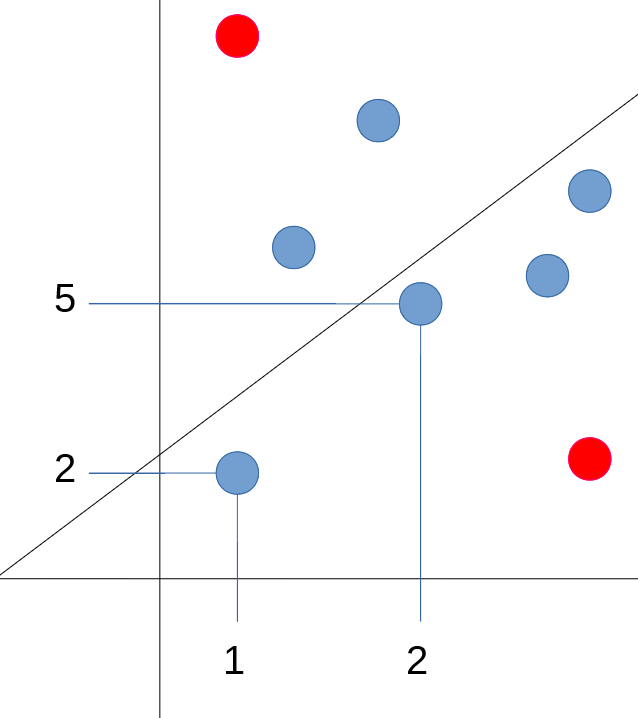
\includegraphics[scale=0.3]{img/ap-linear-regression_1.png}
$Figure ap-linear-regression_1$

\begin{description}
\item[Avec]: y  = $\beta_0 + \beta_1 x$
\item[Pour un hyperPlan (3d)]: y = $\beta_0 + \beta_1 x_1 + ... \beta_n x_n$
\end{description}

Exemple:
\begin{description}
\item[5] =  $\beta_0 + 2 * \beta_1$
\item[2] =  $\beta_0 + 1 * \beta_1$
\end{description}

\pagebreak
\subsection{Least squares linear regression}
Calculer la régression linéaire avec la méthode Least squares:\\
Soit:
\begin{description}
\item[X] = $[1,2,3,4,5]$ les variables indépendantes d'axe abscisse
\item[Y] = $[2,4,5,4,5]$ les variables dépendantes d'axe ordonnée
\item[Calculons] $y = \beta_0 + \beta_1 x$
\end{description}
Calcule de la moyenne de X et Y:
\begin{description}
\item[Xm] = $ \sum x_i \in X$ = 3
\item[Ym] = $ \sum y_i \in Y$ = 4
\end{description}
Toutes ligne de régression doivent passer par le point (Xm,Ym).\\
Calculer tout les écarts des $x_i \in X$ par rapport à Xm (resp Y):\\

\begin{tabular}{ll|l|l|l|l}
  \hline
  X  & Y & $X - Xm$ & $Y - Ym$ & $(X-Xm)^2$ & $(X-Xm)(Y-Ym)$\\
  \hline
  1 & 2 & -2 & -2 & 4 & 4\\
  2 & 4 & -1 & 0  & 1 & 0\\
  3 & 5 & 0  & 1  & 0 & 0\\
  4 & 4 & 1  & 0  & 1 & 0\\
  5 & 5 & 2  & 1  & 4 & 2\\ 
  \hline
\end{tabular}

\begin{description}
\item[$Calculer \beta_1$]:
\item[$ \beta_1 $] = $ \frac{ \sum (X-Xm)(Y-Ym)}{ \sum (X-Xm)^2}$ = $\frac{6}{10}$ = $.6$
\item[$ \beta_0 $]: $Ym = \beta_0 + \beta_1 * Xm$ : $4 = \beta_0 + .6 * 3$ : $4= \beta_0 + 1.8$ : $\beta_0 = 2.2$
\end{description}
\pagebreak
\subsection{Gradient Descent}
Soit:
\begin{description}
\item[X] = $[1,2,4,3,5]$
\item[Y] = $[1,3,3,2,5]$
\item[i] = une variable qui itère les éléments de X et Y en bouclant à l'infini.
\end{description}
Une initialisation comme:
\begin{description}
\item[$\beta_0$] = 0
\item[$\beta_1$] = 0
\item[$\alpha$] = donnée en énoncé (pour l'exemple égal à 0.01)
\end{description}
Et des fonctions définit tel que:
\begin{description}
\item[error] = $(\beta_0 + \beta_1 * X[i]) - Y[i]$
\item[$\beta_{0_{+1}}$] = $\beta_0 - \alpha * error$
\item[$\beta_{1_{+1}}$] = $\beta_1 - \alpha * error * X[i]$
\end{description}

En appliquant l'algorithme des calcules des $\beta_i$:\\
\begin{tabular}{l|l|l|l|l|l}
  \hline
  $ i $ & $ X[i] $ &  $Y[i] $ &  $error $ & $ \beta_0 $ & $ \beta_1 $\\
  \hline
  0 & 1 & 1 & -1 & 0.01 & 0.01 \\
  1 & 2 & 3 & -2.97 & 0.06 & 0.03\\
  2 & 4 & 3 & -1.77 & 0.18 & 0.06\\
  3 & 3 & 2 & -1.61 & 0.22 & 0.08\\
  4 & 5 & 5 & -4.35 & 0.44 & 0.12\\
  0 & 1 & 1 & -0.42 & 0.45 & 0.13\\
  1 & 2 & 3 & -2.28 & 0.49 & 0.49\\
  \hline
\end{tabular}
\pagebreak
\section{Logistic Regression}
\subsection{Logistic function}

Soit:
\begin{description}
\item[t] $\in \Re[0,1]$ égal à $\beta_0 + \beta_2 * x$
\end{description}

La fonction de logique de régression, les valeur d'entrée X sont combiné en utilisant les coefficient de valeur pour prédire une sortie Y. Cette sortie sera une valeur binaire.

\begin{description}
\item[$p(x)$] = $ \frac{1}{1 + e^{-(\beta_0 + \beta_1 * x}}$
\item[Note]: $p(x)$ peut être interprété comme une fonction de probabilité $P(X) = P[Y=1 | X)$.
\item[$\beta_0 + \beta_1 * x$] = $ ln(\frac{P(x)}{1 - P(x)})$ aussi appelé odds.
\end{description}

\subsection{Logistic regression predicts probabolities}


\pagebreak